%  !TeX  root  =  user_guide.tex

\section{Plugin Offline Editing}\label{sec:offlinedit}

% when the revision of a section has been finalized, 
% comment out the following line:
%\updatedisclaimer

In progetti di acquisizione dati è situazione comune trovarsi a lavorare sul 
campo con computer portatili e palmari: i dati in tal modo acquisiti vanno, poi, 
sincronizzati con la banca dati principale, es. un database PostGIS.
Se più persone lavorano simultaneamente sullo stesso set di dati, risulta 
difficile aggiornare la banca dati principale manualmente.

Il plugin \toolbtntwo{offline_editing_copy}{Offline Editing} permette di automatizzare 
l'attività di sincronizzazione, copiando il contenuto della banca dati principale 
(solitamente un database PostGIS o un WFS-T) in un database spatialite e memorizzando 
le modifiche non in linea in tabelle dedicate: le modifiche, poi, vengono sincronizzate una 
volta riconnessi alla rete.

\minisec{Utilizzo del plugin}

\begin{itemize}
\item Aprire alcuni layer vettoriali, es. da PostGIS o da un WFS-T
\item Salvare il progetto
\item Cliccare su 'Converti ad un progetto offline' e selezionare i layer da salvare. 
\item Modificare il layer in modalità non in linea.
\item Riconnetersi alla rete e caricare le modifiche con \toolbtntwo{offline_editing_sync}{Sincronizza}.
\end{itemize}

\begin{figure}[ht]
   \centering
   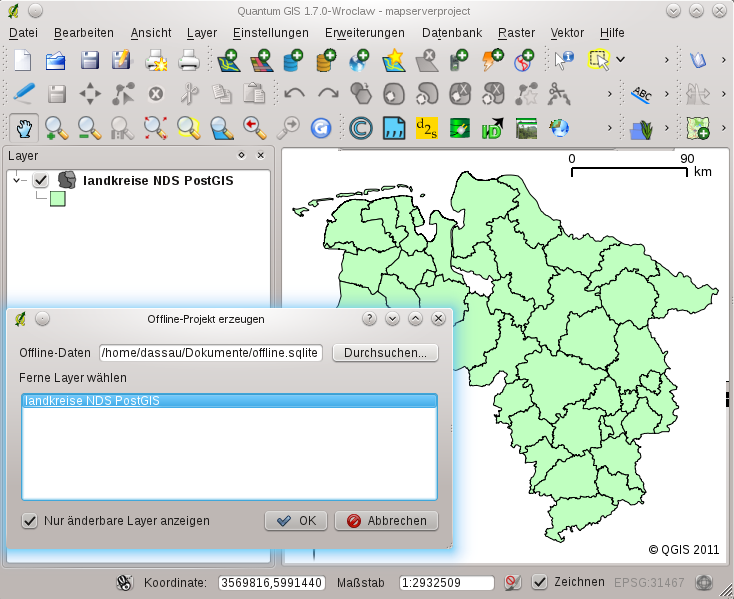
\includegraphics[clip=true, width=12cm]{create_offline_project}   
   \caption{Creazione di un progetto non in linea da layer PostGIS o WFS \wincaption}
   \label{fig:offlineproject}
\end{figure}

\FloatBarrier
